%Introduction

The human brain can be analyzed from different points of views. Some disciplines look at it from the outside, and try to understand how it responds to stimuli, how it behaves on different conditions, how it adapts to new contexts and how it changes over time. Some disciplines look at it at cellular and molecular levels, trying to understand the chemical reactions that go on inside each cell making it work. Others analyze the activity of a groups of cells to explore how they cooperate. Some focus on larger structures composed of several cells, trying to understand how they connect to each other and how the different types of organs complement each other. There is great interest in exploring how the brain matures over time, and how it recovers from traumatic events. Additionally it is important to analyze how it degenerates over time, and what diseases can affect it in order to create treatments and help the brain heal. 
These tasks are carried out by different specialists in very different environments. There are also a wide range of tools designed for studying the brain, from microscopes and voltage clamping techniques, to psychological instruments. There are also studies based on animals with similar structures or even electronics circuits specifically built to emulate the human brain. 

This diversity shows that understanding the brain is far from easy, and that it involves an enormous amount of skills, tools and knowledge. It is also clear that  information gathered from different perspectives must be integrated in other to get a full understanding. This often requires teams from diverse specialties and contexts to work together, each providing one piece of the puzzle. 

This task will also require support from computational tools in order to be efficient. These tools should allow experts from different contexts to be productive as teams and to integrate data acquired using a wide array of methods. Data itself will be highly heterogeneous and there will be lots of it. As tools advance researchers become more efficient at making experiments and generating data, and the bottleneck has become analyzing it. In other words, data is acquired at a faster rate than it can be understood. 

This is indeed a complex scenario, and it is evident that a single software tool will not be able to solve all the problems. Tackling the whole problem at once is also an impossible tasks. A promising approach is to break the problem into simpler tasks that can be attacked without loosing the big picture. However this is itself a challenging task. Fortunately these kinds of problems are found in several business applications and  software engineering techniques can be applied to manage them have been developed. 

As mentioned previously, the problem of integrating brain data involves several points of view and several types of work-flows. This is a clear signal of the need for different applications instead of a single, all encompassing application. Nevertheless these applications will likely share several aspects. Analyzing these commonalities and differences is the first step towards a solution to the problem. 
Methodologies to do this can be borrowed from software product line engineering \autocite{pohl_software_2005}, model driven software engineering \autocite{brambilla_model-driven_2012} and generative programming \autocite{czarnecki_generative_2000}. 

The first task will be the scoping of the domain and the definition of a subdomain in which it is feasible to make a contribution. Afterwards the commonalities and differences in the needs of the different stake-holders, work-flows, and data in the selected domain are analyzed in order to create a feature model. This model will be the basis for a proposal of an applications family, where each application addresses a particular problem inside the domain. 


\section{Domain Engineering}

Domain Engineering is the practice of selecting and characterizing the domain in which the application family will be built. A good description of the steps required for this task can be found in \autocite{czarnecki_generative_2000}. The following describes how this process is used to identify the specific application domain to be addressed by this research.

\subsection{Domain Scoping}

As noted previously brain research involves several specialties, skills and techniques. It could be argued that because the brain is involved in almost every human action, all human and social sciences are at essentially studying the brain. However this effort will focus on direct studies of the human brain; in particular on facilitating exploration of the relationships between cognitive function and the brain's physical structure. Even with this initial definition, however, there are still many ways to scope the application domain.

In domain engineering the decision of where to focus must be driven by the strengths and experience of the organization, in this case, IMAGINE, VRAC and CNS. Previous projects of the group (\footnote{Proyectos de Darwin, Jaime, Marcela}) have principally focused on analysis of medical images at millimeter scale, acquired by CT and MRI machines. The team has good relationships with radiology departments at several hospitals and therefore has access to images and, more critically, domain experts. MRI is an specially interesting technique as it does not produce ionizing radiation, and therefore is harmless for the subject. In contrast CT and general x-rays involve radiating the human body. This is not harmful at small doses but the effects may accumulate over time. Therefore these techniques must be used with care and only when there is a valid medical reason that justifies it. On the other hand, MRI scans can be applied to any subject and there is no need for a medical justification (but the study must typically be approved by an ethics committee). MRI scanners are also versatile machines which can acquire numerous kinds of images. Structural images can be acquired at different configurations which provides better contrast for different tissues or molecules. Advanced techniques provide the ability to do spectroscopy in order to characterize the composition of specific areas of the brain. By using contrast agents it is also possible to precisely locate specific proteins, cells or structures. 
For these reasons the group chose to focus development on images acquired by MRI. We also chose to focus on T1 and T2 weighted structural images, diffusion weighted images and BOLD f-MRI. This decision was motivated by the previous experiences in the group, with the understanding that domain definition and scoping is an iterative process, and this decision can be revisited in the future.

An objective of the project from the start has been the integration of data, therefore in addition to MRI data, which provides structural information, additional data is necessary to provide context and a more complete picture. Recall that a primary  hypothesis of this research is that the brain is better understood by teams of specialists who can bring different perspectives. This leads to the fundamental  challenge of linking the structure and function of the brain. Brain function may signify quick reactions to stimuli, like catching a ball, to complex social behaviors over several years. This kind of data can be collected by economists, psychologists, epidemiologists, and sociologists among others. This information can be very complex, but a non-trivial subset of it can be characterized by numerical, nominal and ordinal variables which can be registered in spreadsheet tables. Thus, the application domain must encompass this type of tabular data. 

Finally data from TMS exams \autocite{nollet_transcranial_2003} is important to consider as it provides a perfect link between structure and functioning of the brain. This is, data from TMS exams. In this technique a fast magnetic pulse is applied outside the skull, which induces an electric field inside the brain. This field can have different effects on the underlying neurons. For example a pulse in the motor region will cause a signal to be send to the corresponding muscle. This electric signal can be measured at the muscle, which allows physiologists to infer the speed and quality of the transmission from brain to muscle. This project is fortunate to have access to neurophysiologists specialized in these kinds of exams. 

To recapitulate, the current project considers the following kinds of data:

\begin{itemize}
\item MRI brain images
\begin{itemize}
\item Structural T1 and T2 weighted
\item Diffusion Weighted Images
\item Functional MRI
\end{itemize}
\item TMS exams
\item Tabular data from other disciplines
\begin{itemize}
\item Nominal variables
\item Ordinal variables
\item Numeric variables
\end{itemize}
\end{itemize}  

Another key aspect of domain scoping is identifying stakeholders and their interests. As mentioned earlier the brain can be studied from a clinical perspective with the aim of healing it. This is usually done case by case in hospitals or health centers. However, addressing the clinical diagnosis practice would involve dealing with significantly more regulations, which would increase the complexity of the project. The other major group of users of medical images are brain researchers. As was described in the introduction, these users are generally interested in analyzing cohorts of subjects (rather than individuals), and are the primary target user community. In particular this research focuses on interdisciplinary brain research projects, where there is data from multiple subjects and different nature, and the user community seeks to find relationships across the different dimensions and disciplines. The data available for each subject should be reasonably consistent across the complete sample. The stakeholders are therefore the researchers involved in such a project. These researchers can come from several backgrounds, including

\begin{itemize}
\item Radiologists
\item Physicians
\item Neonatologists
\item Psychologists
\item Physiologists
\item Epidemiologists
\item Economists
\end{itemize}

The overall goal of such an interdisciplinary team can be characterized generally as  extracting information and meaning out of the data. As mentioned earlier this is the core problem that lead to the birth of visual analytics. However it is crucial to understand that each specialist will inevitably have his or her  own interests and methods. The real challenge is creating a common framework that would help and encourage specialists from different disciplines to work together and collaborate efficiently. To achieve this goal it is necessary to improve communication inside the team, and to encourage specialists to go out of their typical comfort zone and pose questions about data they would not normally ask. However this must be done responsibly, the goal is to improve communication within the interdisciplinary team without hindering the contribution or expertise of individual specialists.

Each specialty also brings its own work-flows. These include protocols for data acquisition, pre-processing, storage, processing and analysis. As mentioned in the introduction analysis usually take the form of null hypothesis significance testing, and plenty of tools exist for this purpose. Nonetheless exploratory data analysis is also very important, especially when huge amounts of data are available. Traditionally data acquisition was also tuned for the testing of particular hypotheses, but it is becoming common to acquire data in a more open-ended fashion. This project will not address data acquisition nor data processing. The focus is on visual exploratory analysis of already processed data.  

In conclusion, the scope of the project is now bounded in data types (MRI and tabular), stakeholders (interdisciplinary research groups), and tasks (visual exploratory analysis). However, it is worth reiterating that domain scoping is an iterative process, which must continue for the duration of the project. 

% Domain Model

%- Stakeholders
%- Users
%-- points of view
%-- activities
%-- teams
%-- selfish
%
%-- Alternatives
%-- choose
%- Scope
%-- Alternatives
%-- Choose


\subsection{Domain Modeling}

After choosing and bounding the domain the next step in its characterization is modeling. This task is accomplished by reading relevant literature in the domain, interviewing stakeholders and analyzing existing software. The details of the information gathered at this stage are described in chapter \ref{chap_related}. In this section the application domain will be further defined and modeled based on that information.

%Workflow
A typical MRI experiment starts with a set of hypotheses to be tested on a target population. A protocol is designed to test the hypotheses, and if, possible correct sample sizes are calculated. Then, participants are recruited and data is collected. This process is not always smooth, and often corrections must be made and acquisition repeated. Inevitably some data will not be useful and some participants will have to be removed from the study. Data acquired from the MRI machine must be acquired, stored and processed. There are different processing pipelines for different kinds of images, but most of them are designed to perform statistical tests using the images and some external variables. The results of the statistical tests must be interpreted in order to write the report of the experiment and what was learned from it.

As mentioned in chapter \ref{chap_intro} the goal to use data collected in these types of experiments as well as data collected in open-ended fashion to perform exploratory and data-driven analyzes. Of course, most of the steps in traditional experiments will be the same, and the proposal should be compatible with them. 

\begin{figure}
\centering
\begin{subfigure}[b]{\textwidth}
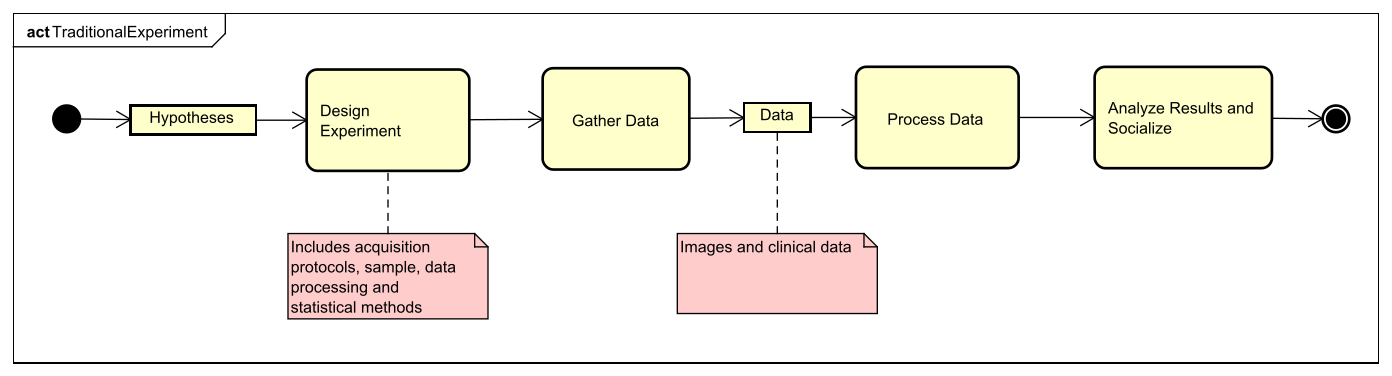
\includegraphics[width=\textwidth]{domain/TraditionalExperiment}
\caption{The Scientific Method workflow}	
\end{subfigure}

\begin{subfigure}[b]{\textwidth}
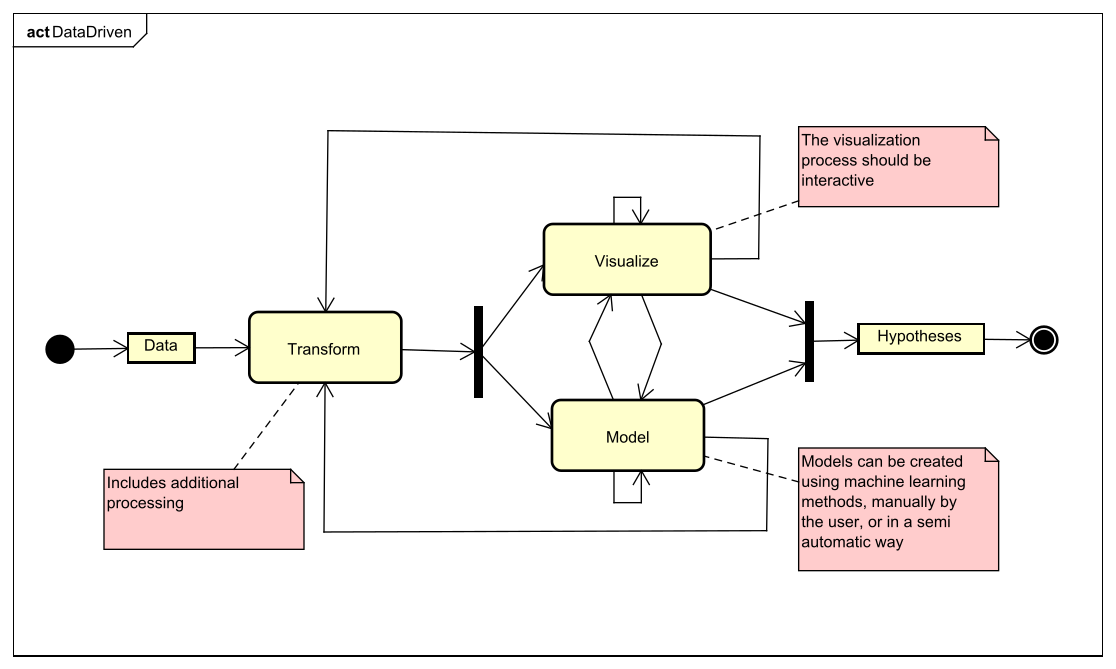
\includegraphics[width=\textwidth]{domain/DataDriven}	
\caption{The Data Driven workflow}	
\end{subfigure}

\caption{\label{fig_workflows}Comparison between scientific method and data driven research.}
\end{figure}

Figure \ref{fig_workflows} shows a comparison of the two work-flows. Notice that the input for traditional experiments are hypotheses, while the output of data driven research are  hypotheses. Notice also that the input to the data-driven research loop is data, which as mentioned earlier, can come from finished experiments. This shows how both work-flows can complement each other. Finally data processing clearly takes place at both both work flows, which indicate that the data-driven and hypotheses-driven research domains are deeply linked.  

%Data
\begin{figure}
\centering
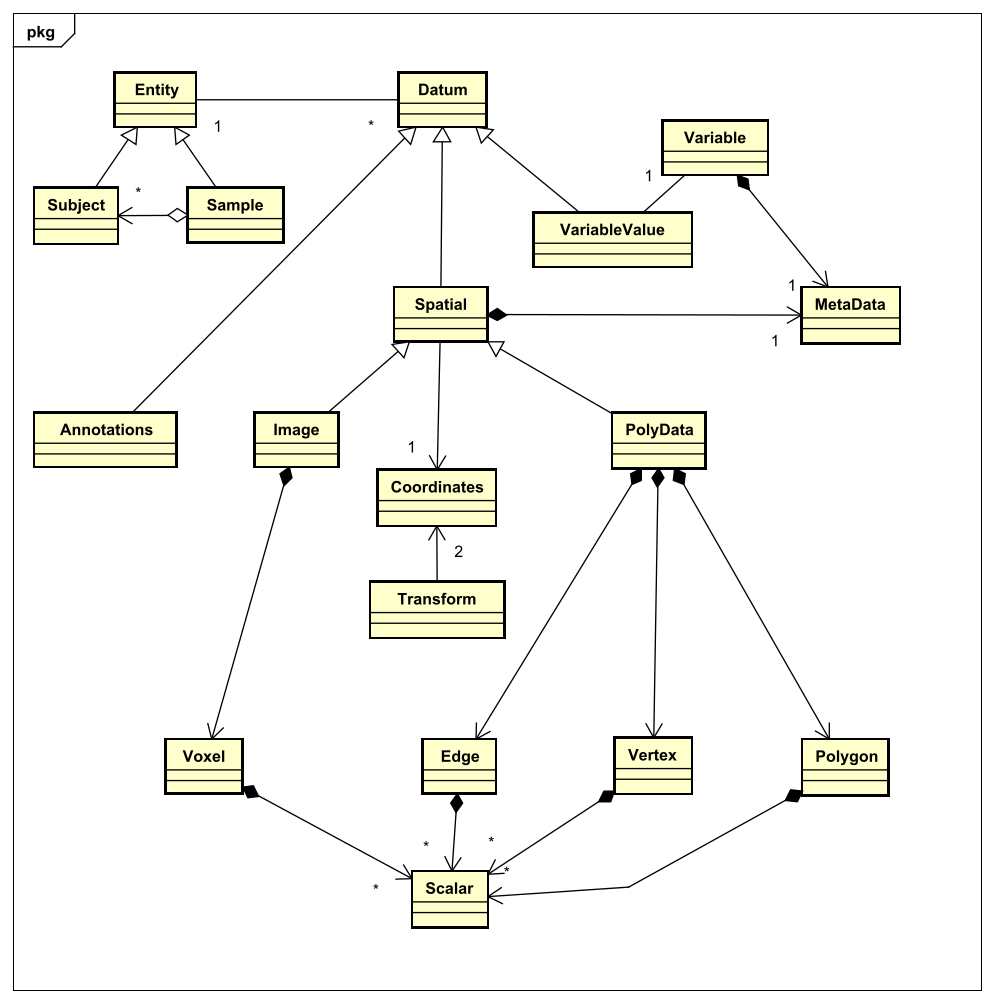
\includegraphics[width=0.9\textwidth]{domain/ClassDiagramData}
\caption{\label{fig_datum_class} Domain data model.}
\end{figure}

Since data is clearly one of the most important objects in the domain, it is necessary to characterize it in a more precise way. Thus in this work, data is defiend as a collection of elements, each of which is called a datum. Figure \ref{fig_datum_class} shows a class diagram of a datum. The highlights of this data definition are

%definitions

\begin{itemize}
\item Each datum is associated to an Entity
\item An entity may be a single subject or a sample
\item A sample is composed of several subjects, each subject can belong to several samples
\item The two main kinds of datum are spatial and variable values
\item An spatial datum may be an image or polydata
\item All spatial objects are associated with a coordinates system
\item Transforms can be used to map between two coordinate systems
\item Images are composed of voxels
\item Polydata are collections of vertices, edges and polygons
\item Voxels, edges, vertices and polygons may be associated with one or more scalar values.
\item All spatial data must be associated to some meta-data
\item VariableValues belong to a certain variable
\item Each variable is associated with meta-data  
\item Data which is neither a VariableValue nor a spatial object can be encoded into textual annotations
\end{itemize} 

Some concrete examples of data are
\begin{itemize}
\item Image:
\begin{itemize}
\item T1-weighted structural image
\item Color coded DTI image with 3 scalar values per voxel
\item A label map where each voxel contains a value indicating to what structure it belongs 
\end{itemize}
\item PolyData:
\begin{itemize}
\item A group of fibers from a tractography
\item Cerebral cortex surface reconstruction
\item An iso-surface representing an activated area in a fMRI paradigm
\end{itemize}
\item Variable:
\begin{itemize}
\item Gender
\item Height
\item Score at a neuropsychological test
\item Time it took to complete a marathon
\item Level of pain in a likert scale
\item Place of birth
\item Latency in a TMS test
\end{itemize}
\end{itemize}

Meta-data plays an important role. On the spatial side it enables identification of which images or polydata can be analyzed together. In other words, metadata makes it possible to identify matching pieces of information belonging to different subjects. In the case of variables, the metadata provides important information on how to interpret the values that the variable takes. 
%Processing

This simple structure allows representation of a wide array of data types. Some of this data are raw values that are obtained directly, and some are the results of processing steps applied to raw data. As mentioned earlier the system is not designed to do data processing, but there is a close relationship with these kind of procedures. In fact the system should be able to do additional processing when it is required, but delegating this task to third party tools is usually appropriate. As shown in figure \ref{fig_workflows} processed data is fed back into the system, and afterwards can be used in the same way as raw data. Some examples of the processing steps that are expected to be utilized are:

\begin{itemize}
\item Estimating diffusion models (like DTI)
\item Reconstructing tractographies
\item Segmentation of structural images
\item Reconstruction of segmented structures
\item Cortical surface reconstruction and parcellation
\item Linear and non linear registration
\item Applying transforms to move spatial objects to a different coordinate system
\item Creating frequency maps from several co-registered label maps.
\item Filtering tractographies
\item Calculating volumes, areas, and mean values of a scalar, for a given surface.
\item Statistical tests involving images from two different groups (like VBM, or second level fMRI analysis)
\item Clustering on a set of variables
\item Fitting of statistical models on a set of variables
\end{itemize}

As usual, this is not an exhaustive nor final list; as the project evolves it is likely that additional processing algorithms will be integrated. The vision is to take advantage of available tools whenever possible. Fortunately there is an ample set of high quality open source tools available as was described on Chapter \ref{chap_related}.

%Stake Holders

The expected users in this project are research groups comprised of specialists from different backgrounds, however several other stakeholders must be considered in the development of the project. The data comes from real participants, and they may have concerns about the privacy and use of their data. On the other hand the project managers and funding agencies want the best return on investment possible, which means extracting as much information and knowledge from the collected data. Usually the participants of the experiment sign a consent which permits some use of the data. The contents and permissions granted by these agreements have to be taken into account. A common trade-off is for the participants to grant unlimited usage of the data as long as it is anonymized. In theory it shouldn't be possible to determine the true identity of a subject based on anonymized data, but this is hard to guarantee in practice, especially when so much complementary data can be obtained from third parties \autocite{singel_netflix_2009}. Also the anonymization procedure involves adding noise to the data, which may have an impact on the analysis. When data is analyzed as extensively and deeply as proposed here, the risk of deanonimyzing the subjects increases. Therefore measures have to be taken to increase protection, either by limiting access to the data to a small group of researchers, or increasing the strength of anonymization measures. 

Another possible concern is the loss of statistical rigor. As shown in figure \ref{fig_workflows} traditional research is based on the fact that data is used once for a statistical test so that meaningful metrics of significance can be reported. However when data is used more than once a multiple comparisons problem can arise in which the chances of false positives increase and therefore corrections should be applied to significance metrics. Nevertheless the scientific community is concerned that this corrections will not be used and false discoveries will be published. While dishonest researchers can not be thwarted by a software tool, the proposed platforms may make it easier to cheat in order to get more impressive results. As mentioned in the introduction, this problem arises from publication bias. Under this situation some researchers may believe that the best way to guarantee a publication is by reporting some fantastic significance metrics, and try everything they can to get these values. It is key here to remember that the proposed platform is meant to be used as a means for generating hypotheses, not to formally prove them. While the analysis carried on in the platform may provide evidence in favor of some hypothesis, it is also highly susceptible to the multiple comparisons problem. Therefore it is necessary to be skeptical about the data, and always validate hypotheses with new data.  

Understanding the main users of the application is at the core of the design process. Recall that a user centered design methodology is undertaken in this work, involving end-users constantly during the design process. Understanding the users is also central for the domain-modeling activity. This begins with examining their current workflows and tools. This was accomplished by visiting several labs and hospitals, and observing several experiments, from data acquisition to data analysis. The knowledge from other works in visual analytics can also be applied here. 

First of all, brain researchers are human and this have limitations on the amount of information that can be kept in memory as well as the length of time one can concentrate. The analysis platform should help mitigate this by unloading the memory of the specialist by making all of the required information visible or easy to access. In order to avoid distractions, it is important to have a fast response time. If the application constantly makes the user wait, then probably he may loose interest and move to another task. A peculiarity of brain researchers is that they are very busy, and usually there is no time in their agenda reserved for data exploration. This activity is carried on in the spaces between tasks, and there is a high chance of being interrupted by students or colleagues. Therefore it is essential for the platform to support work at different intervals and under constant interruptions. In practice this means efficient facilities to save and restore work, as well as additional information to recover the flow from the last session. 

Visual Analytics recognizes that humans have limited cognitive capacity, and the point is to make the best possible use of it, in particular, that the cognitive budget should be spent on the data and not on the tools. This means that the experts should always be thinking about the underlying data, not on details of the tool used to look at it. If tools require complex commands, or the controls are not intuitive, user attention may have to shift to how to accomplish a task in the tool. Another key concept required here is that tools should adapt to users, instead of making users adapt to tools \autocite{norman_design_2002}. This means that technical details or repetitive actions should be easy to automate. For example there are dozens of image data formats available, and each tool works with some of them. This forces the user to spend time to consider which tool is appropriate for each format, or if there is a need to convert it. The same issue applies in dealing with files in file system: users should not required to determine what is the best way to organize files so that they can be easily found afterwards. 

Of course the researchers are the most capable of interpreting and making sense of  vast amounts of data and as the number of dimensions grows larger, the likelihood of patterns appearing by chance increases. Only experts can discriminate between trully interesting findings and random noise. They can do this because they possess a strong theoretical background, which can be used to give meaning to data. They also have experience working with patients and data, and therefore can associate data from a study to past experiences and similar cases. All of these factors combined can lead to  intuition, that can guide experts to interesting places. Given the familiarity with the data, experts can quickly spot common mistakes or find simple explanations to what may appear surprising for an outsider. 

In summary some of the main characteristics of a hypothetical user are

\begin{itemize}
\item Limited memory
\item Limited concentration
\item Busy schedule
\item Not interested in technical details
\item Background knowledge
\item Experience
\item Intuition
\end{itemize}

%Group memebrs also belong to other groups

%Florero, evidencia de los argumentos, no recurrir a la memoria, sino tener la informacion visible

% groups

Groups of experts are also interesting because their expertise is generally in different areas. Therefore while they are deeply familiar with some aspects of the data, other aspects may be foreign. In a similar way each expert is inclined to analyze data of a particular nature or in a particular way. Some teams are composed of experts located far from each other. They may not even share the same mother language. Communication between the different members of the group is therefore challenging, as is reconciling their interests and objectives, and moving forward as a group. Communication is different when a link to the physical reality can be stablished \autocite{rojas_arredondo_dinamica_2010}. By having data easily available at a meeting, researchers can provide evidence to support their ideas, and in this way have a conversation rooted to reality, instead of relying on memory or notes. Also ideas or questions that come up during the conversation could be explored right away, which can lead to a more fluent and efficient work session. Visual analytics recognizes the human visual system as the most effective channel to get information into the expert's mind. Communication can be improved by using this channel efficiently. Also providing easy access may lower the resistance of experts to explore data from other fields , to follow-up with colleagues and bring them questions. Of course, given this functionality, some members of the group want more control of their data, and my not like the idea of non-experts looking at it because they may not understand it. Thus it will be important to evaluate how these kind of tools may affect group dynamics.


\bigskip

% Existing viualization applications
In chapter \ref{chap_intro} a review of the tools currently used in the domain was presented. These tools have several things in common and several differences as shown in table \ref{tab_related_applications}. While most of the processing tools provide utilities for batch processing several subjects, visualization tools generally support viewing data for a single subject or for the results of statistical tests. Going through visualizations of several subjects requires several steps and most of the time repeating work. Also while most of them permit the use of affine transformations to move the data to a different coordinate system, the end user must specify the adequate transform for each case. These tools offer very good performance for quality control or publication graphs, but for exploratory analysis a more streamlined workflow is required, with minimal need for repetition, and limiting as much as possible the exposure of technical details to the user. 

In the world of information visualization there has been a bigger growth in interactive solutions. For example Tableau \autocite{hanrahan_tableau_2003} can be used to create highly interactive dashboards for the exploration of large datasets. These dashboards display several coordinated views of the data and permit the user to interactively change parameters and therefore get visualizations tailored for the current question. One goal of this work is to use these kinds of techniques but extend them to be better integrated with spatial data. 



\bigskip

In summary, the target domain is characterized by
\begin{itemize}
\item Data Sources
\begin{itemize}
\item Spatial Data
\item Tabular Data
\end{itemize}
\item Visual Analytics
\begin{itemize}
\item Data Transformations
\item Fast iteration
\item Interactive Visualizations
\item Focus on data, not tools
\end{itemize}
\item Research groups
\begin{itemize}
\item Collaboration
\item Interrupted work
\item Diverse points of view
\end{itemize}
\end{itemize}

The overall objective is to create a family of applications that can adapt to different tasks inside the domain. Following visual analytics principles these applications should put the data at front, and let users focus on it instead of the applications. For these reasons applications should be simple, and have a limited set of features. Nevertheless to foster collaboration it is important that applications inside the family integrate well with one other. It is also important that applications provide capabilities the user save and restore work efficiently, and therefore work over several interrupted sessions. Figure \ref{fig_use_case_general} shows an overview of the activities to be completed by users in the domain.

The explore activity (Figure \ref{fig_use_case_explore}) can be achieved through a combination of several analysis tasks.
\begin{itemize}
	\item Connect: show similar data
	\item Reconfigure: change arrangement of data
	\item Compare: view differences and similarities between two entities
	\item Drill Down: Get additional details
	\item Group: join similar entities
	\item Annotate: attach additional information to an entity
	\item Aggregate: show less detail
	\item Change: show something different
	\item Filter: show something conditionally
\end{itemize}
 Most of these tasks are taken from \autocite{yi_toward_2007}. The review and share use cases include the following activities. 
\begin{itemize}
	\item BackTrack: reconstruct a previous session
	\item Retrieve: recover the state of a previous section
	\item Send: send data from a previous section to a colleague or a report
\end{itemize}
Finally some applications in the family should support data processing. These applications should enhance data in order to allow additional exploration paths in the next iteration. Examples of this are extraction of scalars from spatial data, either manually, semi-automatically or fully automatically. Another example is aggregating spatial or non-spatial data in order to perform group analyzes.
 
Visualization is the basis of exploratory analysis, and therefore it will likely be at the core of most applications in the family. The set of applications that will constitute part of the family are represented the feature diagram of figure \ref{fig_feature_problem}.

\begin{figure}
\centering
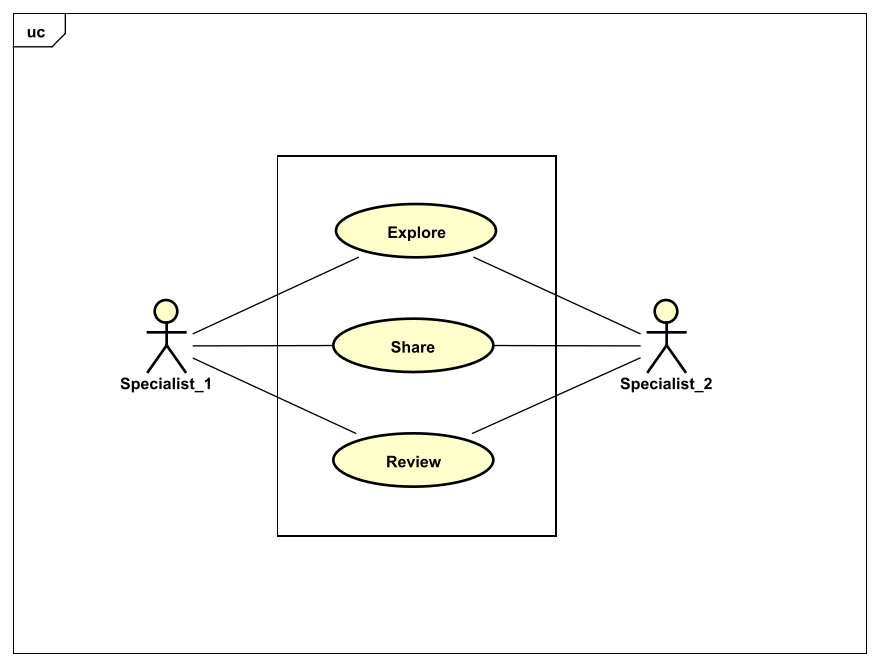
\includegraphics[width=0.7\textwidth]{domain/UseCaseGeneral}
\caption{The high level use cases of the system. It should allow each specialist to explore, share and review. Notice one expert may review the results from another member of the team.\label{fig_use_case_general}}
\end{figure}

\begin{figure}
\centering
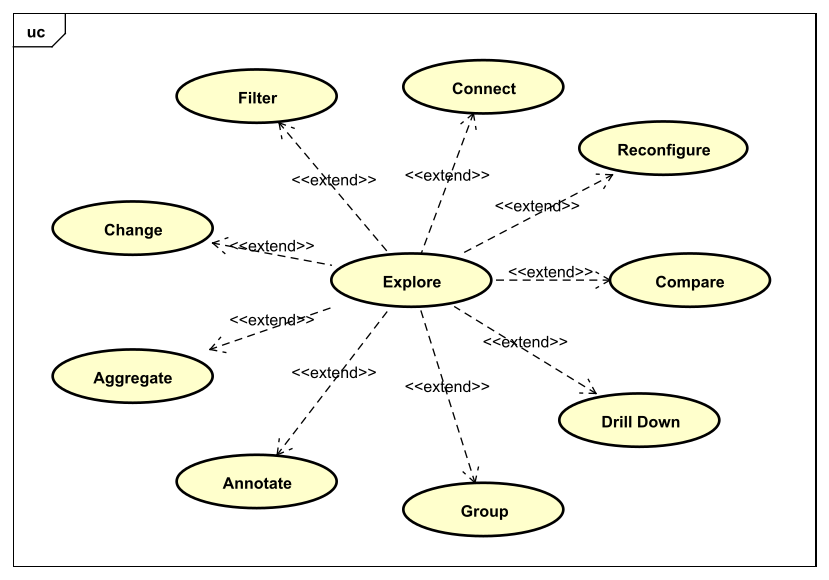
\includegraphics[width=0.9\textwidth]{domain/UseCaseExplore}
\caption{Activities that support data exploration\label{fig_use_case_explore}}
\end{figure}

\begin{figure}
\centering
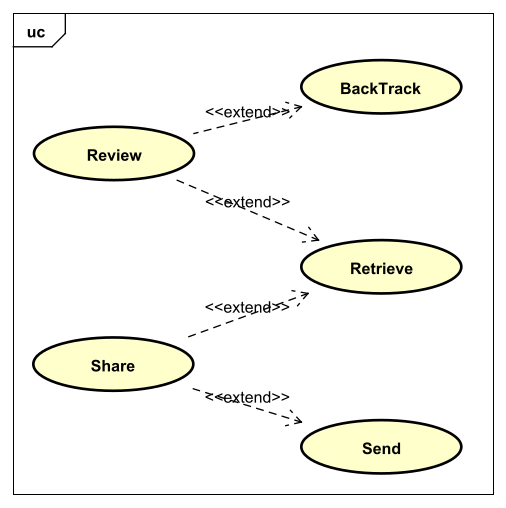
\includegraphics[width=0.6\textwidth]{domain/UseCaseShare}
\caption{Activities that support reviewing and sharing.\label{fig_use_case_share}}
\end{figure}

\begin{figure}
\centering
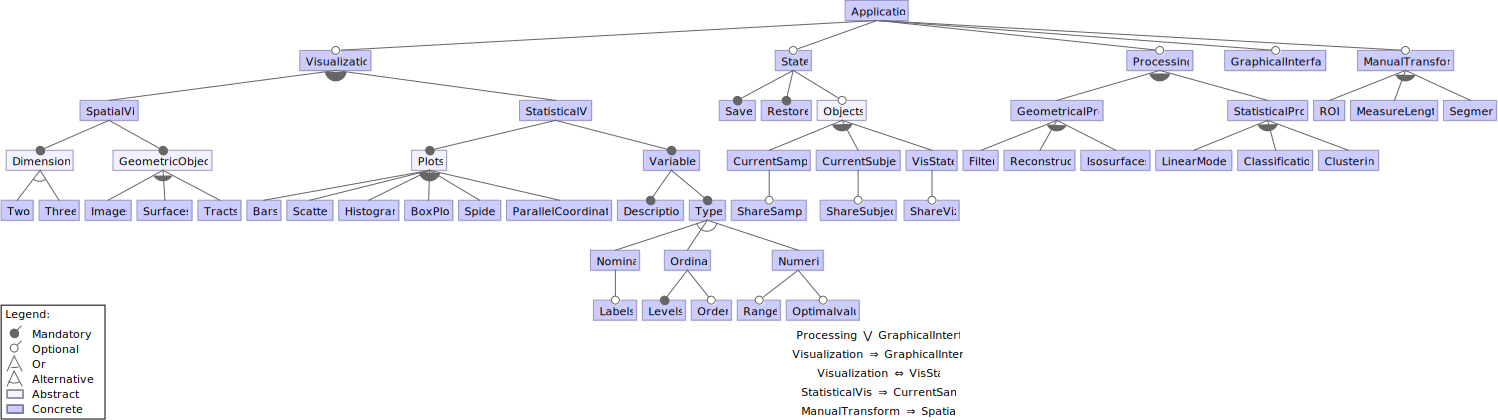
\includegraphics[width=\textwidth]{featureProblem}
\caption{\label{fig_feature_problem}Feature map of the problem space. It illustrates the different features that make up applications for the domain.}
\end{figure}

The main elements in the diagram are:

\begin{itemize}
\item Application: The root of the tree, each of the applications in the family are configured based on this tree
\item Interactive Visualization: Most applications will have interactive functionality as a main component. The exception are applications that prepare data for exploratory analysis. Visualizations can exist for spatial data (usually referred to as scientific visualizations ) or non spatial data (usually referred to as information visualization).
\begin{itemize}
\item Spatial Visualization: These visualizations show spatial objects, this is, objects with coordinates associated to some physical space. Notice this visualizations can be in a plane, with only two coordinates, or a in a full 3d space. These visualizations can display one or several of the listed Geometric Objects.
\item Non-Spatial Visualizations: These visualizations represent abstract values in a coordinate system that is not necessarily associated with any physical space, for example scatter plots, and bar plots. Notice that several of them can be displayed at the same time in order to convey additional aspects of the data. This is especially useful if different views are coordinated. The information displayed in the plots comes from variables. 
\end{itemize}
\item Workflow: Features in this branch are intended to make the exploratory analysis workflow more efficient. 
\begin{itemize}
\item Save Restore: One of the key requirements is being able to split an analysis sessions between several times. Therefore applications should save and restore any state. The state can reference the current subject, current sample and the internal state of visualizations. 
\item Log: Applications may write important actions performed by the user to a log. This log can be further improved with textual comments and highlights written by the user. It can be used afterwards to retrieve the process at a later time or to share with colleagues.
\item Communication: Different applications can communicate with each other in order to provide coordinated views from different points. In this way applications can share a subject of interest, a sample of interest, variables of interest or the configuration of spatial visualizations.
\end{itemize}
\item Interface: Most applications are expected to have a graphical interface so that users can interact with it visually. These interfaces should be simple and expose only the functionality required for a specific task. However some applications can be used to process data in batch form, in order to prepare it for future analysis. In this case a command line interface may be sufficient. 
\item Processing: One of the key steps in the visual analytics loop is data transformation. These transformations can be fully automatic and therefore calculated without the need for user intervention; others will require the intervention of experts.
\begin{itemize}
\item Automatic: These functions may operate on spatial data, and therefore come from the computational geometry domain, or they may operate on tabular data using techniques from statistics or machine learning. Some examples of these operations are shown in the tree.
\item  Manual Assist: Some operations can not be performed reliably in a fully automatic way. In these cases it is necessary to involve the expert in the systematic transformation of the data. Tools should be designed to make the manual intervention as minimal as possible, and everything that could be automated should be in order to ease the workload of the expert. An example could be providing an initial estimation automatically and then let the expert make adjustments. Some examples of these operations are presented in the tree: ROI (Region of Interest) definition, length measurement, and manual segmentation.

\end{itemize}

\end{itemize}

Some additional restrictions can be found at the bottom of figure \ref{fig_feature_problem}. Of course interactive visualizations require a graphical user interface. Manual data transformations are designed for spatial data, and therefore it is mandatory to provide an spatial data visualization.

This feature model represents a family of applications that can be adapted for several tasks, data types and users. Different exploratory workflows can be supported by different configurations. Specifically there are applications focused on transforming the data and others focused on visualizing it. Both of these fit at different places of the visual analytics workflow (figure \ref{fig_workflows}). Notice that the model permits applications focused on spatial data, applications focused on tabular data, but also applications that integrate both of them. The \emph{communications} nodes in the tree allow users and teams to use several applications to complete more complex analyzes. However coordinating operations is more easily accomplished by having a central coordinator. This central coordinator can also help with the recovery of a previous session by keeping a log of the usage of different applications. The following section addresses how this platform and the family of applications can be implemented.

% Commonalities and differences in these applications

% Domain Terms

% Use cases

% Feature model


%- Define domain
%-- Examples
%-- Main Features
%-- Relationship to other domains
%- Analysis of existing Applications
%-- Commonalities and Differences
%-- From other domains, need to be compatible
%- Analysis of literatures and experts
%- Domain Terms
%- Domain Concepts
%- Variability of domain concepts
%-- feature model in problem space
% trade offs
% analyzis of combinations

\section{Solution Proposal}

The domain described above requires applications tailored for specific tasks and data, but also requires the integration of data, users and workflows. In order to achieve this, a family of applications and a common platform that integrates them is proposed. Because target users have to do exploratory research through several small sessions spread through a long time, it is critical that the system helps them pick up work where they left off. Additionally it is crucial to document findings, so that they can be corroborated and socialized. This requires the association of a finding with the data that supports it, as well as how it is made evident through the right visualizations. The path to such a finding or insight may involve going through several applications. These applications also need to be coordinated in order to make moving from one to the other pleasant, avoiding the need to repeat tasks and therefore allowing the expert to concentrate more easily. Thus, a node is proposed to coordinate communication between applications and keep a log of the activity of all of them. This log can be improved with annotations from the user, and reviewed at any time. Specific elements from the log can be shared to colleagues and associated to findings. The diagram in figure \ref{fig_deployment} shows the processes that compose the proposed system.

The \emph{Main Menu} process behaves as the master of the session. A single database containing all data and is accessible by all applications. Any derived data is sent to this same database. This shared database is the first mechanism for coordination between applications, but more fluid integration can be achieved by sharing state information across the system. For this purpose all applications connect to the \emph{Main Menu}. A delegate of this central application keeps track of important changes done on the other applications and saves them into a dedicated log database. This log allows future retrieval and reconstruction of the analysis session.

\begin{figure}

\centering
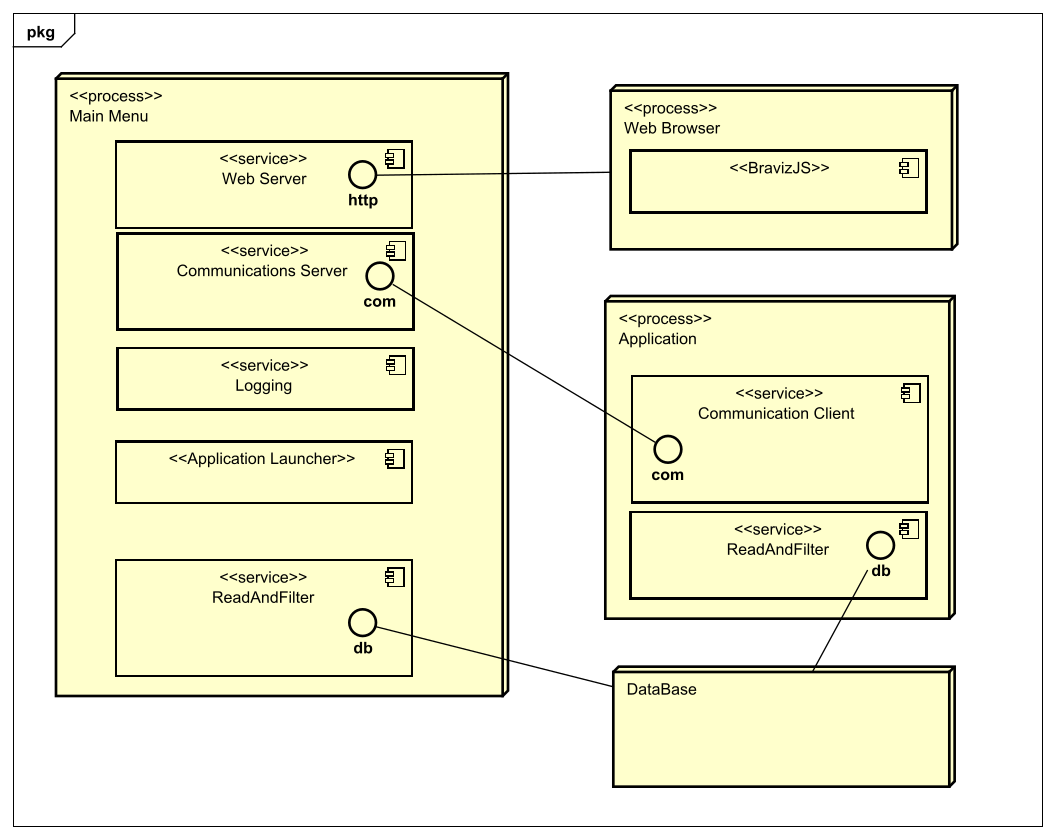
\includegraphics[width=\textwidth]{braviz/BravizDeploy}
\caption{\label{fig_deployment} Deployment diagram of the proposed solution. At the left is the main process, which includes the communication server and logger, to the right there are web-based applications that run on a web server as well as desktop applications each one running on its own process. Notices that all of them share the same database.}
\end{figure}
 
It can be seen that individual applications support the \emph{explore} use case, while the platform plays the main role in \emph{share} and \emph{review}. The next chapters describes an implementation of the proposed system and how it gets used in real projects.

\subsection{Platform}

Exploratory analysis requires iterating through the data several times, using different tools to explore relationships, trends or contrasts. This is best accomplished by using different that provide complementary functionality  enhanced via seamlessly shared data. This research proposes a set of coordinated applications for this task. Usually changing from one application to another requires a relatively high cognitive overhead. For this reason users try to avoid switching applications, and when it has to be done, they are forced to change their focus to the details of the operation and momentarily forget about the data. The environment proposed in this research allows users to move seamlessly between applications. Even better, multiple applications can be opened at the same time, and input in one will be reflected on the other. If large display real estate is available, there may be multiple application and thus, multiple  points of view active at the same time, so the specialist can scan the displays to see the current data from a different point of view. Even though work happens on several different applications, the overall user experience is coherent work-flow. 

During the visual analytics cycle shown in figure \ref{fig_workflows} data is constantly transformed and fed back into the process. In the proposed analysis environment there is a single pool of data. All applications read data from it, expose it to the user, and in case the user requests a transformation, the transformed data is fed back into the system. In this way the pool of data is constantly growing and getting richer. This data created by one application can be accessed from any other. This provides a practical mechanism to move data between applications. 

Data in this domain is either associated with an individual subject or to a group (see figure \ref{fig_datum_class}). During an analysis session users will look at several subjects of groups. Each application provides a different way to look at this subjects or groups. Some focused on spatial data while others will focus on complementary data. The mechanism through which this is achieved is that when an application changes the current sample or subject, it reports the change to the rest of the running applications. These applications listen to the message and react. If applications behave in unexpected ways, they may confuse the user, who may not understand what is going on. Then it is important to make explicit the messaging mechanism, and let the user turn it on, off or fine tune it at will. This mechanism can improve user experience by providing the user the information he is interested in at the right time.

 Events of the entire system of federated applications is monitored by the central position of the message server. Applications not only send reports when switching focus, but also send messages reporting changes in their internal states  for logging purposes. The purpose of the log is to let users review the workflow and especially the path that led to a discovery. For this reason it is important to display this log to the user in a way that facilitates recollection of the situation or workflow at a glance. The log should also allow annotations such that it can be shared among users. Finally, the crucial pieces of evidence that support a discovery should be identifiable from the log, associated to the discovery and finally attached to a report on such discovery.



%Proposal for Braviz platform
%
%- Data Flow
%- Task
%- Use Case (igual que arriba?)
%- Deployment


\subsection{Applications Family}

The goal is to support a very diverse set of applications that adapts to several users and tasks. While each application serves a different purpose, there are all based on common functionality. This work uses echniques from Software Product Line Engineering \autocite{pohl_software_2005} as they provide a framework to efficiently develop several applications based on common functions but explicitly supporting points of variability. The feature diagram from figure \ref{fig_feature_problem} show the expected variability from the user perspective. From it a second feature plot (see figure is dervied \ref{fig_feature_solution}) that shows this variability from a more technical point of view.  

\begin{figure}
\centering
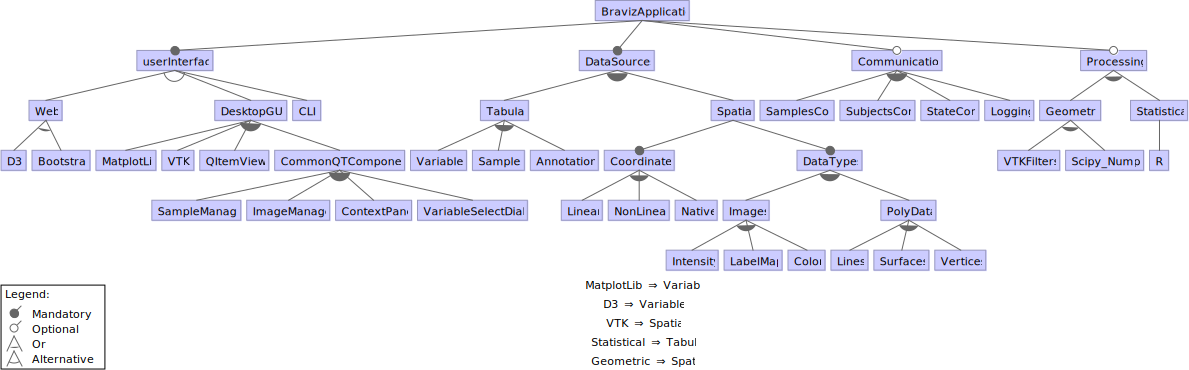
\includegraphics[width=\textwidth]{featureSolution}
\caption{\label{fig_feature_solution}Feature Diagram of the solution space. It shows the available choices of features to create applications in the domain. Choices must be made depending on the task and the user.}
\end{figure}

Notice that this diagram indicates some of the specific technology selections that will be used in the implementation. For example VTK \autocite{schroeder_vtk_1998} is the most common scientific visualization framework, and many existing scientific visualization tools are built using it. Given that a primary objective of this work is to leverage existing software resources this is as a natural choice. On the statistical side, R \autocite{team_r:_2012} is one of the most widely used statistical tool, and it has the advantage of being open source. This enables easy  application development and integration, without imposing a financial burden on the user community. Python is adopted as the main development environment, again, because it has become one of the most popular languages in the neuro-science  community. This facilitates linking several packages to perform data processing and reading. An important example is the nipy \autocite{gorgolewski_nipype:_2011-1} suite. There are also robust scientific libraries \autocite{van_der_walt_numpy_2011, jones_scipy:_2001,mckinney_data_2010} available in Python as well as libraries for statistical plotting, for example Matplotlib \autocite{hunter_matplotlib:_2007} and seaborn \autocite{michael_waskom_seaborn:_2015}.

Most of the proposed applications require a graphical user interface. Two alternatives are proposed for implementation, a web-based user interface or a standalone client. Web interfaces can provide high quality interactive graphics using java-script libraries such as D3 \autocite{bostock_d3_2011}, it is also possible to show 3d graphics on web browsers using \emph{webgl} and related libraries such as \emph{three.js}. However these technologies are still very young and experimental. In contrast, interactive 3D graphics in a desktop client is a mature technology. Additional user interface elements can be created using the QT framework on desktop and the bootstrap and d3 frameworks on the web. The decision between web and desktop must be made based on the kind of visualization that the application will contain. In general, if complex interactive 3d graphics are required, a standalone desktop client is currently the most reliable option.Common components have been implemented in this work and are available for all applications to reuse. At the current stage these are

\begin{itemize}
\item SampleManager: Handles creation, loading, saving and optionally communication of samples.
\item ImageManager: Allows the user to select an image from the collection of images available in the current project.
\item ContextPanel: A panel that displays values of selected variables for the current subject.
\item VariableSelectDialog: A generic dialog that lets the user search and select variables, as well as review and modify the associated meta-data.
\end{itemize}


In general, each application requires different data sources. The possible sources are classified in two groups, namely spatial and non-spatial. Non-spatial data is further categorized as variables, samples or annotations. 
Variables represent properties of the subjects or samples, and therefore generally have a description to help with its interpretation. There are three main types of variables.
\begin{itemize}
\item Nominal Variables: These variables represent categories of data. They don not necessarily have an order and in general it is not possible to perform arithmetic operations on them. Examples of these are: Gender, City of birth and eye's color.
\item Ordinal Variables: These variables have an associated order but in general it is not possible to perform arithmetic on them. Examples of these are a Likert scales (e.g, strongly agree, agree, neither agree or disagree, disagree or strongly disagree), months in a year, streets in a city, poker hands or a names in a phone-book.
\item Numerical variables: These variables can me mapped to a subset of the real numbers. They can be further divided into \emph{interval} and  \emph{ratio}. In interval data the distance between two values is meaningful, for example temperature in degrees Celsius, dates or coordinates in the globe. These variables can be added and subtracted, and statistics like the arithmetic mean and variance are meaningful. Ratio variables additionally have a meaningful zero or origin. Examples of these are age, speed, height, weight or electric field. It makes sense to multiply two of these values together and therefore statistics like the geometric mean are meaningful.
\end{itemize}

Samples are grouping of subjects which can be used to test a hypothesis only for a specific group, or to compare several groups. Annotations are free-text complementary information on each subject or sample. They can be used to store and keep present information that can not be encoded into variables.

The other main data type is  spatial data. These can be Images or PolyData structures, and they may be required in one or more coordinate systems. There are three possible kinds of images: intensity, in which each voxel contain a real number indicating the intensity of a signal or effect; label map, in which each voxel contains an integer representing membership to a set; and color images, in which each voxel contains a color. Polydata may contain vertices, lines or surfaces. Additionally there may be scalar values associated to each vertex, line, or polygon. 

Spatial data my be shown on a single coordinate system, or the user may have the option to select the best one for the current task. Usually there is a trade-off. Native coordinate systems display data as it was acquired, and therefore provide the highest fidelity. Linear registration requires resampling, which can add noise to the data; however it is easier to make comparisons on registered data. Finally non-linear registration provides the highest correspondence between data from different subjects, but adds a significant amount of distortion. This space may be adequate when one wants to compare scalar values at a given location on different subjects, however most of the differences in shape or size will disappear.

Communications mechanisms are optional. But including them allow for more fluid collaboration. Communication may include sending and receiving samples, subjects, complete state or logging messages. The later are interpreted by the logging module in the central node. Finally applications may include facilities to transform and process data. Statistical processing can be done using R, while geometrical processing can be accomplished using either VTK or the python scientific libraries Numpy and Scipy which provide several geometry, linear algebra, optimization and statistics algorithms. 

It may be tempting to create applications that include all possible features, however most likely this will result on overly complex applications which are hard to use. Applications should generally be designed to target a concrete task. Features should be added only when they help accomplish the task. Features should not be added just because they can be added. Simplicity plays a key role. 

Notice that while there is significant room for variability across applications, it is expected that they all share a large amount of code. By doing this critical pieces of code  can be implemented and tested once, and then used across the different applications. The result is that application developers only need to worry about the target user and task; while technical details are handled by the reusable components. This separation of concerns enables development of several distinct applications designed for specific analysis tasks and users, on top of a solid shared foundation. More details about the implementation of the system are described on chapter \ref{chap_braviz}.


%Proposal for Braviz application family
%
%- Feature model
%-- problem space
%-- solution space
%
%- rationale for each choice
%- when to select each feature
%- how to choose between alternatives